% Options for packages loaded elsewhere
\PassOptionsToPackage{unicode}{hyperref}
\PassOptionsToPackage{hyphens}{url}
%
\documentclass[
]{article}
\usepackage{lmodern}
\usepackage{amssymb,amsmath}
\usepackage{ifxetex,ifluatex}
\ifnum 0\ifxetex 1\fi\ifluatex 1\fi=0 % if pdftex
  \usepackage[T1]{fontenc}
  \usepackage[utf8]{inputenc}
  \usepackage{textcomp} % provide euro and other symbols
\else % if luatex or xetex
  \usepackage{unicode-math}
  \defaultfontfeatures{Scale=MatchLowercase}
  \defaultfontfeatures[\rmfamily]{Ligatures=TeX,Scale=1}
\fi
% Use upquote if available, for straight quotes in verbatim environments
\IfFileExists{upquote.sty}{\usepackage{upquote}}{}
\IfFileExists{microtype.sty}{% use microtype if available
  \usepackage[]{microtype}
  \UseMicrotypeSet[protrusion]{basicmath} % disable protrusion for tt fonts
}{}
\makeatletter
\@ifundefined{KOMAClassName}{% if non-KOMA class
  \IfFileExists{parskip.sty}{%
    \usepackage{parskip}
  }{% else
    \setlength{\parindent}{0pt}
    \setlength{\parskip}{6pt plus 2pt minus 1pt}}
}{% if KOMA class
  \KOMAoptions{parskip=half}}
\makeatother
\usepackage{xcolor}
\IfFileExists{xurl.sty}{\usepackage{xurl}}{} % add URL line breaks if available
\IfFileExists{bookmark.sty}{\usepackage{bookmark}}{\usepackage{hyperref}}
\hypersetup{
  hidelinks,
  pdfcreator={LaTeX via pandoc}}
\urlstyle{same} % disable monospaced font for URLs
\usepackage{color}
\usepackage{fancyvrb}
\newcommand{\VerbBar}{|}
\newcommand{\VERB}{\Verb[commandchars=\\\{\}]}
\DefineVerbatimEnvironment{Highlighting}{Verbatim}{commandchars=\\\{\}}
% Add ',fontsize=\small' for more characters per line
\newenvironment{Shaded}{}{}
\newcommand{\AlertTok}[1]{\textcolor[rgb]{1.00,0.00,0.00}{\textbf{#1}}}
\newcommand{\AnnotationTok}[1]{\textcolor[rgb]{0.38,0.63,0.69}{\textbf{\textit{#1}}}}
\newcommand{\AttributeTok}[1]{\textcolor[rgb]{0.49,0.56,0.16}{#1}}
\newcommand{\BaseNTok}[1]{\textcolor[rgb]{0.25,0.63,0.44}{#1}}
\newcommand{\BuiltInTok}[1]{#1}
\newcommand{\CharTok}[1]{\textcolor[rgb]{0.25,0.44,0.63}{#1}}
\newcommand{\CommentTok}[1]{\textcolor[rgb]{0.38,0.63,0.69}{\textit{#1}}}
\newcommand{\CommentVarTok}[1]{\textcolor[rgb]{0.38,0.63,0.69}{\textbf{\textit{#1}}}}
\newcommand{\ConstantTok}[1]{\textcolor[rgb]{0.53,0.00,0.00}{#1}}
\newcommand{\ControlFlowTok}[1]{\textcolor[rgb]{0.00,0.44,0.13}{\textbf{#1}}}
\newcommand{\DataTypeTok}[1]{\textcolor[rgb]{0.56,0.13,0.00}{#1}}
\newcommand{\DecValTok}[1]{\textcolor[rgb]{0.25,0.63,0.44}{#1}}
\newcommand{\DocumentationTok}[1]{\textcolor[rgb]{0.73,0.13,0.13}{\textit{#1}}}
\newcommand{\ErrorTok}[1]{\textcolor[rgb]{1.00,0.00,0.00}{\textbf{#1}}}
\newcommand{\ExtensionTok}[1]{#1}
\newcommand{\FloatTok}[1]{\textcolor[rgb]{0.25,0.63,0.44}{#1}}
\newcommand{\FunctionTok}[1]{\textcolor[rgb]{0.02,0.16,0.49}{#1}}
\newcommand{\ImportTok}[1]{#1}
\newcommand{\InformationTok}[1]{\textcolor[rgb]{0.38,0.63,0.69}{\textbf{\textit{#1}}}}
\newcommand{\KeywordTok}[1]{\textcolor[rgb]{0.00,0.44,0.13}{\textbf{#1}}}
\newcommand{\NormalTok}[1]{#1}
\newcommand{\OperatorTok}[1]{\textcolor[rgb]{0.40,0.40,0.40}{#1}}
\newcommand{\OtherTok}[1]{\textcolor[rgb]{0.00,0.44,0.13}{#1}}
\newcommand{\PreprocessorTok}[1]{\textcolor[rgb]{0.74,0.48,0.00}{#1}}
\newcommand{\RegionMarkerTok}[1]{#1}
\newcommand{\SpecialCharTok}[1]{\textcolor[rgb]{0.25,0.44,0.63}{#1}}
\newcommand{\SpecialStringTok}[1]{\textcolor[rgb]{0.73,0.40,0.53}{#1}}
\newcommand{\StringTok}[1]{\textcolor[rgb]{0.25,0.44,0.63}{#1}}
\newcommand{\VariableTok}[1]{\textcolor[rgb]{0.10,0.09,0.49}{#1}}
\newcommand{\VerbatimStringTok}[1]{\textcolor[rgb]{0.25,0.44,0.63}{#1}}
\newcommand{\WarningTok}[1]{\textcolor[rgb]{0.38,0.63,0.69}{\textbf{\textit{#1}}}}
\usepackage{longtable,booktabs}
% Correct order of tables after \paragraph or \subparagraph
\usepackage{etoolbox}
\makeatletter
\patchcmd\longtable{\par}{\if@noskipsec\mbox{}\fi\par}{}{}
\makeatother
% Allow footnotes in longtable head/foot
\IfFileExists{footnotehyper.sty}{\usepackage{footnotehyper}}{\usepackage{footnote}}
\makesavenoteenv{longtable}
\usepackage{graphicx}
\makeatletter
\def\maxwidth{\ifdim\Gin@nat@width>\linewidth\linewidth\else\Gin@nat@width\fi}
\def\maxheight{\ifdim\Gin@nat@height>\textheight\textheight\else\Gin@nat@height\fi}
\makeatother
% Scale images if necessary, so that they will not overflow the page
% margins by default, and it is still possible to overwrite the defaults
% using explicit options in \includegraphics[width, height, ...]{}
\setkeys{Gin}{width=\maxwidth,height=\maxheight,keepaspectratio}
% Set default figure placement to htbp
\makeatletter
\def\fps@figure{htbp}
\makeatother
\setlength{\emergencystretch}{3em} % prevent overfull lines
\providecommand{\tightlist}{%
  \setlength{\itemsep}{0pt}\setlength{\parskip}{0pt}}
\setcounter{secnumdepth}{-\maxdimen} % remove section numbering

\author{}
\date{}

\begin{document}

\hypertarget{header-n0}{%
\section{软件学院书籍影视交流平台------软件开发计划书}\label{header-n0}}

\hypertarget{header-n2}{%
\subsection{引言}\label{header-n2}}

a

\hypertarget{header-n641}{%
\subsection{摘要}\label{header-n641}}

a

\hypertarget{header-n638}{%
\subsection{言}\label{header-n638}}

\hypertarget{header-n3}{%
\subsubsection{项目背景}\label{header-n3}}

随着社会的进步和发展,现在人们对生活的追求都逐渐提高,不再局限于一些满足日常需求,开始对精神上的追求引起重视,会不定时的前往电影院观看一部电影,放松身心的同时也收获了快乐与满足,也会偶尔抽空在咖啡馆或者图书室拿起一本心爱的书,静静的品味,任由时间飘荡。还喜欢在互联网上的一些论坛或者博客,发表一些自己对某些影片或者书籍的看法以及体验。人们的阅读热潮和观影兴趣日渐增加,在这样的社会背景下,我们小组决定着手进行一个书籍影视交流平台的开发。

\hypertarget{header-n5}{%
\subsubsection{项目目的}\label{header-n5}}

正如上文所提到,电影和书籍开始在我们现在的生活中变成了必不可缺的一部分,因此各种类似的平台层出不穷,例如知名度很高的豆瓣,以及各类博客网站,都是非常好的平台,因此我们这个项目的目的,并不是为了获得多高的知名度或者造成多大的影响,我们的主要目的是为了了解如何去搭建这样一个平台,如何更好的维护这样一个平台,如何在功能上做得更好,从而促使我们更好的学习发展,更好的了解其中需要的技术,而其平台的影响力就显得次要了。当然目的还有完成课程的任务,这是最浅显的,也是很重要的。

\hypertarget{header-n7}{%
\subsubsection{参考资料}\label{header-n7}}

{[}1{]} 吕云翔.软件工程实用教程{[}M{]}.北京:清华大学出版社,2015.

\hypertarget{header-n9}{%
\subsubsection{相关文档}\label{header-n9}}

{[}1{]} 《需求规格说明书》

{[}2{]} 《软件设计说明书》

{[}3{]} 《部署文档》

{[}4{]} 《测试报告》

{[}5{]} 《用户使用说明书》

\hypertarget{header-n15}{%
\subsubsection{涉及名词解释}\label{header-n15}}

{[}1{]}
用户:包含未注册用户以及已经完成注册的用户,在平台中主要进行交互的对象。

{[}2{]}
小组管理员:指在参与小组中的一个负责的对象,能够对其小组的帖子进行管理。

{[}3{]}
系统管理员:则是指整个平台的管理员,与实际平台的功能等等关联不大。

\hypertarget{header-n19}{%
\subsubsection{版本更新记录}\label{header-n19}}

@版本更新记录表

\begin{longtable}[]{@{}ccccc@{}}
\toprule
版本 & 更新者 & 更新 & 更新纪要 & 完成度\tabularnewline
\midrule
\endhead
v1.0.0 & 杨壮 & 2020.4.12 & 项目创建 & 暂无\tabularnewline
v1.0.1 & 张涵珂 & 2020.4.21 & 引言和安排 & 暂无\tabularnewline
v1.0.2 & 杨哲宇 & 2020.4.22 & 条件和预算 & 暂无\tabularnewline
v1.0.3 & 叶天宇 & 2020.4.22 & 问题分析,计划介绍 & 暂无\tabularnewline
v1.0.4 & 杨壮 & 2020.4.26 & 完善了本文档 & 暂无\tabularnewline
v1.0.5 & 蔡星晨 & 2020.4.26 & 编写了计划部分 & 暂无\tabularnewline
& & & &\tabularnewline
\bottomrule
\end{longtable}

\hypertarget{header-n70}{%
\subsection{项目概述}\label{header-n70}}

\hypertarget{header-n71}{%
\subsubsection{项目目标}\label{header-n71}}

本书籍影视交流平台的目标是加强人与人之间关于书籍和影视的思考和讨论,让人们无障碍地交流书籍与影视,在思考与讨论中迸发出知识的火花。也可以让访客了解并体会书籍和影视作品的艺术感、美感,更加感悟其深度。

本书籍影视交流平台主要包括了资源库、话题、小组的模块。每个模块都有其相对应的主页,用户可以参与书籍影视的评论和反馈,也可以参与话题和小组,发表相关的图片和文字。管理员可以对小组的帖子进行置顶、精华、删除的操作。

\hypertarget{header-n74}{%
\subsubsection{项目范围}\label{header-n74}}

本节主要依照《需求规格说明书》的相关章节来说明该一部分的一些设计范围。

\hypertarget{header-n76}{%
\paragraph{功能模块列表}\label{header-n76}}

功能模块列表如表2.1所示。

\begin{longtable}[]{@{}ccc@{}}
\toprule
模块编号 & 名称 & 模块功能描述\tabularnewline
\midrule
\endhead
101 & 注册 & 游客注册为正式用户\tabularnewline
102 & 登录 & 已注册用户登录系统\tabularnewline
103 & 找回密码 & 已注册用户丢失密码后,通过审核找回密码\tabularnewline
104 & 查看个人信息 & 管理员或者已注册用户查看个人信息\tabularnewline
105 & 修改个人信息 & 已注册用户登陆之后对资料进行管理\tabularnewline
106 & 删除用户 & 管理员删除不合法用户\tabularnewline
201 & 浏览内容 & 游客或者用户浏览网站内容\tabularnewline
202 & 检索内容 & 游客或者用户检索网站内容\tabularnewline
203 & 评论书籍 & 用户对书籍进行打分和评论\tabularnewline
204 & 评论影视 & 用户对影视进行打分和评论\tabularnewline
205 & 点赞评论 & 用户对书籍影视评论进行点赞\tabularnewline
206 & 反对评论 & 用户对书籍影视评论表示反对\tabularnewline
207 & 举报评论 & 用户举报书籍影视评论\tabularnewline
301 & 浏览内容 & 游客或者用户浏览话题内容\tabularnewline
302 & 检索内容 & 游客或者用户及检索话题内容\tabularnewline
303 & 参与话题 & 用户成为某一个话题的参与者\tabularnewline
304 & 创建话题 & 用户创建了一个新的话题\tabularnewline
305 & 发表图文 & 用户在某一个话题下发表相关言论和图片\tabularnewline
401 & 检索内容 & 用户检索小组相关的内容\tabularnewline
402 & 浏览内容 & 用户浏览小组相关的内容\tabularnewline
403 & 创建小组 & 用户创建了一个新的小组\tabularnewline
404 & 参与小组 & 用户成为了某一个小组的参与者\tabularnewline
405 & 发表帖子 & 用户在某一个小组中发表了帖子\tabularnewline
406 & 置顶帖子 & 小组管理员置顶了一个帖子\tabularnewline
407 & 加精帖子 & 小组管理员将某一个帖子设为精华帖\tabularnewline
408 & 删除帖子 & 小组管理员删除了一个非法的帖子\tabularnewline
\bottomrule
\end{longtable}

\hypertarget{header-n187}{%
\paragraph{性能点列表}\label{header-n187}}

性能点列表如表2.2所示。

\begin{longtable}[]{@{}cccccc@{}}
\toprule
编号 & 性能需求来源名称 & 使用者 & 功能描述 & 响应要求 &
结果\tabularnewline
\midrule
\endhead
1 & 查看热点内容 & 游客、用户 & 加载热点图书影视的信息,展示在页面上 &
在1秒内列出所有的内容 & 输出符合要求的记录\tabularnewline
2 & 检索书籍、影视 & 游客、用户 & 通过关键词对书籍影视信息进行检索 &
在1秒内列出所有的内容 & 输出符合要求的记录\tabularnewline
3 & 登录认证 & 游客 & 通过登录账号将身份提升为用户 &
在0.5秒内验证信息,输出提示信息 & 登录到系统\tabularnewline
4 & 信息的修改、录入、删除 & 管理员 & 录入、修改、删除书记影视的信息 &
在0.5秒内刷新数据库,输出提示信息 & 输出提示信息\tabularnewline
5 & 加载页面 & 游客、用户 & 将相关内容加载在页面上 &
在1秒内列出所有的内容 & 输出符合要求的记录\tabularnewline
6 & 发表帖子和内容 & 用户 & 在相关话题和小组内发表图片和文字 &
在0.5秒内刷新数据库,输出提示信息 &
输出提示信息,更新页面\tabularnewline
\bottomrule
\end{longtable}

\hypertarget{header-n239}{%
\subsubsection{项目使用对象}\label{header-n239}}

本平台的最终用户是软件学院师生,若开放则最终用户可以拓展到所有网络用户,使用网络者一般计算机基础都较为扎实,所需硬件设施为连接到互联网的计算机或者智能手机。

系统维护人员为本项目的开发团队,对于此系统的相关部分比较熟悉,团队内部具有对数据库、计算机、网络较为熟悉的人员,维护难度不是很大。

管理员为开发团队指定人员,当规模扩大后的管理员可以由用户投票选出,不需要较强的技术能力。

\hypertarget{header-n243}{%
\subsubsection{预计交付成果}\label{header-n243}}

\hypertarget{header-n244}{%
\paragraph{预计交付的软件}\label{header-n244}}

基于Django和Vue.js开发的``豆辛瓜辛''书籍影视交流平台程序。其中包括由Django开发的后台服务,使用Vue.js编写的前端,基于MySQL构建的数据库系统。

\hypertarget{header-n246}{%
\paragraph{预计交付的文档}\label{header-n246}}

预计共包括以下8个文件

\begin{enumerate}
\def\labelenumi{\arabic{enumi}.}
\item
  《软件开发计划书》
\item
  《需求规格说明书》
\item
  《软件设计说明书》
\item
  《用户使用说明书》
\item
  《部署文档》
\item
  《测试报告》
\end{enumerate}

\hypertarget{header-n261}{%
\subsubsection{项目开发环境}\label{header-n261}}

使用Windows系统进行开发,开发环境如下:

\begin{verbatim}
操作系统:Windows 10 1903
数据库系统:MySQL
IDE:Visual Studio Code
测试工具:Google Chrome
编码方式:UTF-8
\end{verbatim}

\hypertarget{header-n264}{%
\subsection{组织安排}\label{header-n264}}

\hypertarget{header-n265}{%
\subsubsection{团队组成}\label{header-n265}}

各成员基本信息如下:

@成员基本信息表

\begin{longtable}[]{@{}cc@{}}
\toprule
姓名 & 班级\tabularnewline
\midrule
\endhead
杨壮(组长) & 182112\tabularnewline
杨哲宇 & 182113\tabularnewline
张涵珂 & 182113\tabularnewline
叶天宇 & 182113\tabularnewline
蔡星晨 & 182113\tabularnewline
\bottomrule
\end{longtable}

\hypertarget{header-n287}{%
\subsubsection{成员分工}\label{header-n287}}

@成员分工表(未)

\begin{Shaded}
\begin{Highlighting}[]
\NormalTok{这里可以填写项目经理,前端开发,页面设计,前后端交互实现,整体设计,性能保证,后端开发,文档编写(等任务)}
\end{Highlighting}
\end{Shaded}

\begin{longtable}[]{@{}cc@{}}
\toprule
成员 & 主要任务\tabularnewline
\midrule
\endhead
杨壮 & 项目经理,页面设计,前端开发,后端开发,文档编写\tabularnewline
杨哲宇 & 前端开发,后端开发,文档编写\tabularnewline
张涵珂 & 前端开发,后端开发,文档编写\tabularnewline
叶天宇 & 前端开发,后端开发,文档编写\tabularnewline
蔡星晨 & 前端开发,后端开发,文档编写\tabularnewline
\bottomrule
\end{longtable}

\hypertarget{header-n309}{%
\subsubsection{协作与沟通}\label{header-n309}}

\hypertarget{header-n310}{%
\paragraph{协作沟通对象}\label{header-n310}}

几乎每一个成功的项目,都是离不开合作和交流,为了能够让项目更好的完成,也为了提高大家团队协作的能力,需要不定时的进行沟通交流来完善项目。而沟通交流的对象则包括:小组成员(能够保证开发的统一性)、其他小组(通过小组间的沟通合作来检查不足以及参考别人的长处)、课程相关负责人(和老师、助教的交流沟通来确保自己项目的研究方向的正确以及及时询问参考老师的建议,来使项目完成的更好)、项目的参与者(即与平台用户的交流,才能根据反馈更好的完善项目)。

\hypertarget{header-n312}{%
\paragraph{沟通方式}\label{header-n312}}

小组成员内部则使用QQ进行线上交流、通过腾讯会议进行线上会议、在返回学校后可以不定期开展线下会议来讨论进行沟通。平时项目上的细节以及小的疑问就通过线上聊天进行解决。如果有比较大的问题或者有比较重要的需求的确定的时候,可以根据情况进行线上的会议(未返校),或者进行线下的实时会议来解决完成。

与其他小组的交流则还是主要通过线上的聊天和线下的交流进行,借鉴别的小组的长处来时自身完成的更好。

而与课程主要负责人(助教、教师)间的沟通则主要是通过电子邮件、在方便的时候进行线上询问(通过聊天工具)以及在条件允许的情况下进行面对面的交流(返校后)。在项目需要进行一定的整改、项目的一些重要需求不是很确定时与负责人取得联系,及时进行相应的修改。

与项目参与者的沟通则主要是通过平台本身,或者通过用户提供的联系方式进行邮件、短信或者电话的形式来进行。通过反馈及时调整,让平台更加的完善。

\hypertarget{header-n317}{%
\paragraph{协作模式}\label{header-n317}}

小组的协作模式主要是大家一起沟通协调、不以某一方的观点实施,在团队的达成一致的情况下再进行相应的完成,由组长带头进行协商。对于组员的建议以及相关沟通对象的意见,小组一起协商、思考并改进,统一小组内部,才能更好的体现团队的力量,才能更好的完成项目。

\hypertarget{header-n319}{%
\subsection{实施计划}\label{header-n319}}

\hypertarget{header-n320}{%
\subsubsection{风险评估}\label{header-n320}}

作为一个大型工程,书籍影音交流平台的搭建对初次开发大型平台的我们来说不是一个简单的任务。所幸,在互联网上我们可以找到许多的参考资料,帮助我们学习。同时,这也是一次较为经典的软件开发实践,我们可以从中得到很大的磨练。\\
以下几点是我们所考虑的难度与风险:

\begin{enumerate}
\def\labelenumi{\arabic{enumi}.}
\item
  服务器的租用。
\item
  前端与后端的交互,获取服务器数据。
\item
  模块功能的调试测试。
\item
  前端页面的美化设计。
\item
  后端框架设计。
\end{enumerate}

\hypertarget{header-n333}{%
\subsubsection{工期计划}\label{header-n333}}

项目开发时间:2020.04.13-2020.05.27(校历第八周至第十四周)

\begin{longtable}[]{@{}cccccccc@{}}
\toprule
任务编号 & 任务名称 & 工期 & 开始时间 & 完成时间 & 前置任务 & 资源名称 &
完成百分比\tabularnewline
\midrule
\endhead
1 & 项目启动 & 1 个工作日 & 4月12日 & 4月12日 & & 项目团队 &
100\%\tabularnewline
2 & 项目分工 & 1 个工作日 & 4月13日 & 4月13日 & 1 & 项目经理 &
20\%\tabularnewline
3 & \textbf{项目分析} & \textbf{3 个工作日} & \textbf{4月14日} &
\textbf{4月16日} & \textbf{2} & & \textbf{0\%}\tabularnewline
4 & 项目实现方式 & 1 个工作日 & 4月14日 & 4月14日 & & 项目团队 &
0\%\tabularnewline
5 & 项目模块分析 & 1 个工作日 & 4月15日 & 4月15日 & 4 & 项目团队 &
0\%\tabularnewline
6 & 项目页面组成 & 1 个工作日 & 4月16日 & 4月16日 & 5 & 项目团队 &
0\%\tabularnewline
7 & \textbf{项目前后端设计} & \textbf{3 个工作日} & \textbf{4月17日} &
\textbf{4月21日} & \textbf{3} & & \textbf{0\%}\tabularnewline
8 & 项目前端设计 & 1 个工作日 & 4月17日 & 4月17日 & & 前端开发 &
0\%\tabularnewline
9 & 项目后端设计 & 2 个工作日 & 4月17日 & 4月20日 & & 后端开发 &
0\%\tabularnewline
10 & 前后端设计审核 & 1 个工作日 & 4月21日 & 4月21日 & 9 & 项目经理 &
0\%\tabularnewline
11 & \textbf{项目全面开发} & \textbf{20 个工作日} & \textbf{4月22日} &
\textbf{5月19日} & \textbf{7} & & \textbf{0\%}\tabularnewline
12 & \textbf{前端开发} & \textbf{17 个工作日} & \textbf{4月22日} &
\textbf{5月14日} & \textbf{8} & & \textbf{0\%}\tabularnewline
13 & 前端组件绘制 & 3 个工作日 & 4月22日 & 4月24日 & & 前端开发 &
0\%\tabularnewline
14 & 前端代码编写 & 14 个工作日 & 4月27日 & 5月14日 & 13 & 前端开发 &
0\%\tabularnewline
15 & \textbf{后端开发} & \textbf{17 个工作日} & \textbf{4月22日} &
\textbf{5月14日} & & & \textbf{0\%}\tabularnewline
16 & 数据库部分开发 & 3 个工作日 & 4月22日 & 4月24日 & & 后端开发 &
0\%\tabularnewline
17 & 主要功能部分开发 & 14 个工作日 & 4月27日 & 5月14日 & 16 & 后端开发
& 0\%\tabularnewline
18 & 接口实现 & 3 个工作日 & 5月15日 & 5月19日 & 15 & 后端开发 &
0\%\tabularnewline
19 & \textbf{项目功能测试} & \textbf{2 个工作日} & \textbf{5月20日} &
\textbf{5月21日} & \textbf{18} & & \textbf{0\%}\tabularnewline
20 & 功能模块测试 & 2 个工作日 & 5月20日 & 5月21日 & & 项目团队 &
0\%\tabularnewline
21 & \textbf{项目改进} & \textbf{3 个工作日} & \textbf{5月22日} &
\textbf{5月26日} & \textbf{19} & & \textbf{0\%}\tabularnewline
22 & 根据测试进行改进 & 3 个工作日 & 5月22日 & 5月26日 & & 项目团队 &
0\%\tabularnewline
23 & 项目汇总 & 1 个工作日 & 5月27日 & 5月27日 & 21 & 项目团队 &
0\%\tabularnewline
24 & 项目结束 & 0 个工作日 & 5月27日 & 5月27日 & 23 & 项目团队 &
0\%\tabularnewline
\bottomrule
\end{longtable}

\hypertarget{header-n561}{%
\subsubsection{开发流程甘特图}\label{header-n561}}

\begin{figure}
\centering
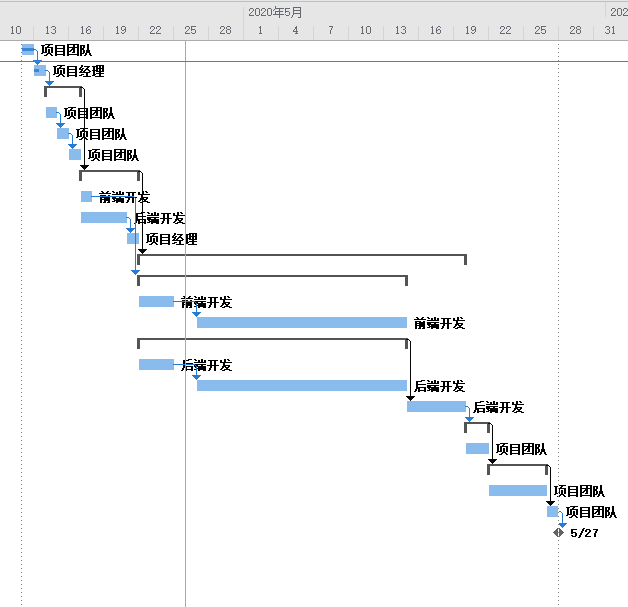
\includegraphics{D:/code/buaase-2020-chatplatform/docs/生成的LaTeX/pic/gant.png}
\caption{}
\end{figure}

\hypertarget{header-n563}{%
\subsubsection{项目控制计划}\label{header-n563}}

考虑到初次合作开发一款软件,其中的难点和盲点我们不容易在一开始就得知,而在项目进行时再临时进行大范围大规模的更改和调度也不够现实。我们认为采取以下措施有利于更好地控制我们的项目进行。

\begin{enumerate}
\def\labelenumi{\arabic{enumi}.}
\item
  在项目开始前成员适度了解相关知识,做好准备,将相应的难度较高的部分进行合理的统筹安排。
\item
  成员间保持时刻联系,做到信息的及时交互,尽量避免因缺少沟通而产生的问题,如软件开发的统一原则,功能模块的设计程度等。
\item
  知悉老师及学长的联系方式,达到一旦陷入无法解决的僵局时有比较可靠的来源进行参考或帮助。
\item
  保证进度的有序进行,定时开会讨论(如一周一次)。
\end{enumerate}

\hypertarget{header-n574}{%
\subsection{支持条件}\label{header-n574}}

\hypertarget{header-n575}{%
\subsubsection{计算机系统支持}\label{header-n575}}

\hypertarget{header-n576}{%
\paragraph{开发}\label{header-n576}}

\hypertarget{header-n577}{%
\subparagraph{硬件}\label{header-n577}}

软件开发使用组员的个人PC机,硬件配置要求参见相关开发软件的硬件需求。

\hypertarget{header-n579}{%
\subparagraph{软件}\label{header-n579}}

代码编辑器:Visual Studio Code

数据库软件:MySQL

UI设计工具:Adobe XD

图像编辑工具:Adobe Photoshop

部署服务器:软件后端的部署需要租用云服务器,我们计划采用阿里云轻量应用服务器(Simple
Application
Server)作为网页后端服务器,该服务器是可快速搭建的轻量级云服务器;提供基于单台服务器的应用部署,安全管理,运维监控等服务。

服务器配置如下:

\begin{itemize}
\item
  1核CPU 2GB内存
\item
  40GB SSD
\item
  5Mbps 峰值带宽
\item
  操作系统:Ubuntu 18.04 LTS
\end{itemize}

数据库:搭建在轻量应用服务器的MySQL服务端,如果遇到性能,存储瓶颈可以考虑增加独立MySQL服务器。如阿里云云数据库RDS
MySQL 版。

存储:用户数据量较小的情况下可以直接使用服务器的40GB
SSD作为存储空间,后期如果存储量变大或者处于可靠、安全性的考虑,可以使用阿里云对象存储(OOS)其具有海量、安全、低成本、高可靠的特点,提供99.9999999999\%的数据可靠性。使用RESTful
API
可以在互联网任何位置存储和访问,容量和处理能力弹性扩展,多种存储类型供选择全面优化存储成本。

CDN:如果用户访问量过高,导致网站难以访问,可以启用CDN服务。CDN将源站内容分发至最接近用户的节点,使用户可就近取得所需内容,提高用户访问的响应速度和成功率。解决因分布、带宽、服务器性能带来的访问延迟问题。

\hypertarget{header-n598}{%
\subsubsection{用户支持}\label{header-n598}}

本平台面向的用户是软件学院的学生,不存在对于网站基本功能使用不熟练的问题,因此无需额外的用户使用培训。对于少数的,如软件bug,用户自身操作失误等引发的问题,我们可以在网站上设立FAQ页面引导用户解决问题。同时还可以设立提问邮箱,用于和用户进行使用问题的沟通。

\hypertarget{header-n600}{%
\subsubsection{外界支持}\label{header-n600}}

本平台为小组人员独立开发,不需要外界提供相关支持。

\hypertarget{header-n602}{%
\subsection{预算预估}\label{header-n602}}

\hypertarget{header-n603}{%
\subsubsection{人员成本}\label{header-n603}}

本项目并非商业项目,开发成员均为课程小组成员,因此不会产生人员使用相关费用。人力使用上,本小组共计5人,预计产品经理一人,美工一人,软件开发两人,软件测试一人。

\hypertarget{header-n605}{%
\subsubsection{设备成本}\label{header-n605}}

在项目开发阶段,主要使用的设备是组员的PC机,因此不会产生额外的费用。

在软件的部署阶段,则产生服务器、数据库、存储空间、CDN等云服务的租用费用,大致估算如下:

\begin{itemize}
\item
  阿里云轻量应用服务器 ¥9.50 /月
\item
  阿里云云数据库MySQL ¥6.90 /月(可选)
\item
  阿里云对象存储标准存储包100GB ¥27.39 /6月 (可选)
\item
  阿里云内容分发网络(中国大陆流量) ¥0.24 /GB(可选)
\end{itemize}

\hypertarget{header-n617}{%
\subsubsection{其他经费预算}\label{header-n617}}

为完成相关项目开发,可能需要学习新的编程语言和软件使用,其中可能产生如购买教材等学习成本。

\hypertarget{header-n619}{%
\subsection{关键问题}\label{header-n619}}

\hypertarget{header-n620}{%
\subsubsection{个性化设计}\label{header-n620}}

为了保证书籍影视交流平台帮助用户找到自己喜欢的书籍影视作品以及向用户推荐其可能感兴趣的内容的功能,在书籍影视交流品台上需要实时的展示当下的热门的相关作品,同时能够根据用户检索的喜好来个性化的推荐与用户通常浏览与访问相关的内容。同时,还设计了话题广场、小组活动板块,使得用户根据自身的需求在不同的话题或小组中找到自己感兴趣的内容。同时,用户可以对相关作评发表自己的感想与心得。

\hypertarget{header-n622}{%
\subsubsection{用户体验}\label{header-n622}}

为了满足用户迅速了解书籍影视作品相关内容的需求,书籍影视平台的UI设计会相对简洁。在设计上会使对书籍影视的评级、小组活动、话题广场等功能的界面简单明了、层次结构清晰。为了方便用户进行对相关作品的了解,对书籍设置了星级评定、评论等功能,对书籍的评论限定在25字符之内,对书籍的评论反馈限定于15字符之内,并且要求著名标题来方便用户能够迅速的对相关内容进行了解。

\hypertarget{header-n624}{%
\subsubsection{平台规范性}\label{header-n624}}

因为书籍影视交流平台需要满足大量用户交流使用,这就需要对平台进行相关的管理,避免用户交流中出现各种违规的现象。所以,在书籍影视管理平台上设置了多种用户的访问权限,分为游客、注册用户、小组管理员。其中游客只能进行对相关内容进行浏览和访问;而注册用户在此之上能够对相关的书籍影视进行评论和反馈的操作,加入相关小组,但同时也只能浏览未加入的小组的帖子;同时,小组成员可以申请小组管理员,还能够对相关的帖子进行置顶、删除、精华等操作。

\hypertarget{header-n626}{%
\subsection{项目计划介绍}\label{header-n626}}

\hypertarget{header-n627}{%
\subsubsection{项目成员培训计划}\label{header-n627}}

鉴于团队相关成员对服务器网站的开发框架以及一些其他的技术难点上的不熟悉,我们考虑在4月12日至5月19日项目开发期间将定期的集体技术培训,融入到项目进程中,以提高团队开发效率,降低之前提到的技术风险。

\hypertarget{header-n629}{%
\subsubsection{项目测试计划}\label{header-n629}}

预计在2019年5月20日-2019年5月21日对本系统进行测试,同时进行相关的改进工作。在5月22日至5月26日对汇总后的平台进行功能测试与改进。

\hypertarget{header-n631}{%
\subsubsection{质量保证计划}\label{header-n631}}

严格按照项目开发过程中的各项步骤,从项目立项,可行性研究报告、需求分析报告、项目开发计划等逐步具体实施。\\
并且在项目开发的每个阶段都进行当前阶段的项目备份,防止由于突发问题导致由于无法还原版本二质量下降。

\hypertarget{header-n633}{%
\subsubsection{安全保密计划}\label{header-n633}}

在从项目开发阶段到最后软件的正式发布期间,做好项目的保密工作,团队所有成员对我们项目的所有开发计划以及相关的文档进行加密,并做好备份工作。

\hypertarget{header-n635}{%
\subsubsection{学习总结计划}\label{header-n635}}

在项目开发过程中,对解决的问题以及学习到的技术点进行汇总记录,并于最后总结为一个学习文档,作为我们团队成员的开发成果,同时也便于大家以后开发项目更好的处理难题。

\end{document}
